\section{Experimental Setup}
\label{sec:setup}

We run two studies. The first is a controlled simulation on four forecasting
tasks. The second repeats the core comparison on real quantum hardware. In both,
every aggregation choice reads the very same measurement record, so any
difference in accuracy comes only from how the shots are organized and not from
running the circuit differently.

\subsection{Simulation reservoir and evaluation protocol}

The simulated reservoir is a fixed six-qubit circuit with two shallow data
reuploading layers~\cite{perezsalinas2020data}. Each layer applies
input-dependent $R_y$ and $R_z$ rotations with fixed per-qubit offsets,
nearest-neighbor $R_{zz}$ couplings, and fixed non-Clifford mixing rotations.
For each circuit setting, all angles are sampled once and then held fixed;
three frozen settings are used to assess sensitivity to this draw. Each
computational-basis shot yields 11 features: six local observables $Z_i$ and
five nearest-neighbor products $Z_iZ_{i+1}$. A leaky integrator with leak rate
$0.2$ and a ten-step lag window provide temporal memory, and a ridge-regression
readout predicts the next value.

We evaluate one-step-ahead forecasting on four time series: the synthetic
Mackey--Glass~\cite{mackey1977oscillation} and
R\"ossler~\cite{rossler1976equation} systems, and the measured Santa Fe laser
intensity~\cite{gershenfeld1993future} and monthly sunspot
number~\cite{sidc2026sunspots}. All tasks use the same reservoir architecture,
feature construction, temporal processing, scaling, validation procedure, and
execution budgets. The same selection rule is applied separately to each task;
no task-specific changes are made to the reservoir or preprocessing pipeline.

All four finite-shot methods use the same measurement record. Two additional
controls use different feature sources: an ideal reservoir without
finite-shot sampling noise and a classical baseline that applies the same
temporal processing and readout directly to the input series. These controls
distinguish the effect of aggregation from the effects of finite sampling and
of the reservoir transformation itself.

The trajectory or time window is the unit of uncertainty estimation.
Mackey--Glass uses twenty independently generated trajectories, each with a
held-out test block. R\"ossler uses five trajectories, and each real-world task
uses five windows with disjoint test blocks.
Within each unit,
we repeat the analysis over three circuit settings, three measurement draws,
and three random groupings where applicable. These repeats are averaged within
the unit before paired confidence intervals are formed across the independent
units for that task.
Grouped views, neighboring time steps, and repeated evaluations of the same
sequence are not treated as independent observations, because they share
measurements or are coupled by the leaky integrator and overlapping lags.

Model selection uses no test data. After a short washout, the final 20\% of each
trajectory or window is reserved as an untouched test block. The preceding
data are used in three expanding-window validation splits, each trained on the
available past and evaluated on the immediately following block. The group
size $k$ and ridge strength $\lambda$ are selected from these validation
results. The readout is then refitted on all data preceding the test block and
evaluated once on the reserved block. For representations with multiple views
at one time step, the corresponding predictions are averaged to produce one
forecast, so all methods are scored on the same targets.

The primary budget uses $T=500$ time steps and $N=20$ shots per step, giving
10,000 circuit executions. We also test $(T,N)=(250,40)$ and $(1000,10)$,
which spend the same budget with different balances between observed time
steps and shots per step. All reservoir parameters, data-generation settings,
window origins, and selection rules are fixed and stored before any test block
is evaluated.

\subsection{Hardware setup}
The hardware study uses a different reservoir: a fixed ten-qubit circuit with
one input qubit, nine memory qubits, a ring of entangling gates, and ten local
outputs mapped on \emph{ibm\_fez} and \emph{ibm\_marrakesh}. It tests transfer of
the aggregation procedure; it is not a hardware implementation of the six-qubit
simulator or a comparison of qubit counts. Every method receives the same
circuit outputs. For each task and processor, one acquisition of $400$ shots at $500$ time steps is
split into twenty ordered, disjoint records of $20$ shots. The intervals measure
variation within that acquisition, not across devices or calibration periods.

\begin{figure}[!t]
  \centering
  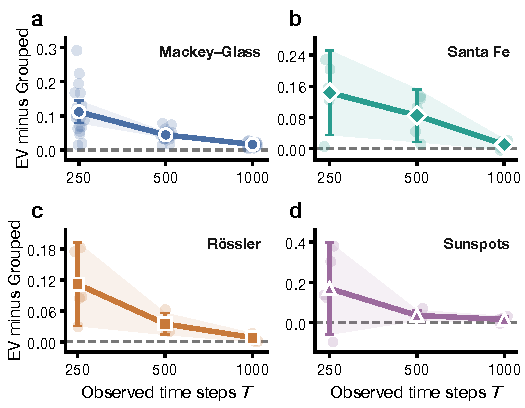
\includegraphics[width=\columnwidth]{fig3_regime_map.pdf}
  \caption{Fixed-budget allocation. Panels show EV-minus-Grouped NRMSE, so
  positive values favor Grouped. Moving right spends the budget on more steps
  and fewer shots; gains are largest with many shots and few steps. Markers and
  bars are means and 95\% intervals.}
  \label{fig:regimes}
\end{figure}
